\documentclass[a4paper, 10pt]{article}
\usepackage{amsmath}
\usepackage{fancyhdr}
\usepackage{float}
\usepackage[a4paper, left=0.9in, right=0.9in, top=0.9in, bottom=0.9in]{geometry} % Adjust margins
\usepackage{graphicx}
\usepackage{listings}
\usepackage{matlab-prettifier}

\pagestyle{fancy}

\title{ECE 340 Lab 4}
\author{Omar Mahmoud\\1753607\\Section D21}
\date{11/18/2024}

\lhead{Omar Mahmoud}
\rhead{ECE 340 Lab 4}
\headheight 15pt

\begin{document}

%% Cover Page
\thispagestyle{empty}
\vfill
\maketitle
\vfill

\newpage

% Q1: Low-Pass Filtering Audio Signals
\section{Low-Pass Filtering Audio Signals}
The script below creates a 513-tap low-pass FIR filter with a cut-off frequency of 2500 Hz and a sampling frequency of
22050 Hz. The truncation window was selected to ensure that the stop-band ripples of the frequency response did not 
exceed -50dB:
\begin{lstlisting}[style=Matlab-editor, basicstyle=\small\ttfamily]
  figure(1);
  fc = 2500;              % Cutoff frequency in Hz
  Fs = 22050;             % Sampling frequency in Hz
  wc = fc / (Fs / 2);     % Normalized cutoff frequency

  % Windowing parameters
  window = hamming(513);   % Hamming window of length 513

  % Design the FIR filter using the fir1 function
  filter_coeff = fir1(513 - 1, wc, 'low', window); % 513 taps, 513 - 1 in the order

  % Plot the frequency response of the filter
  freqz(filter_coeff, 1); % 1024 points for a smooth plot, Fs as sampling frequency
\end{lstlisting}
The code above generates the following frequency response plots:
\begin{figure}[H]
  \centering
  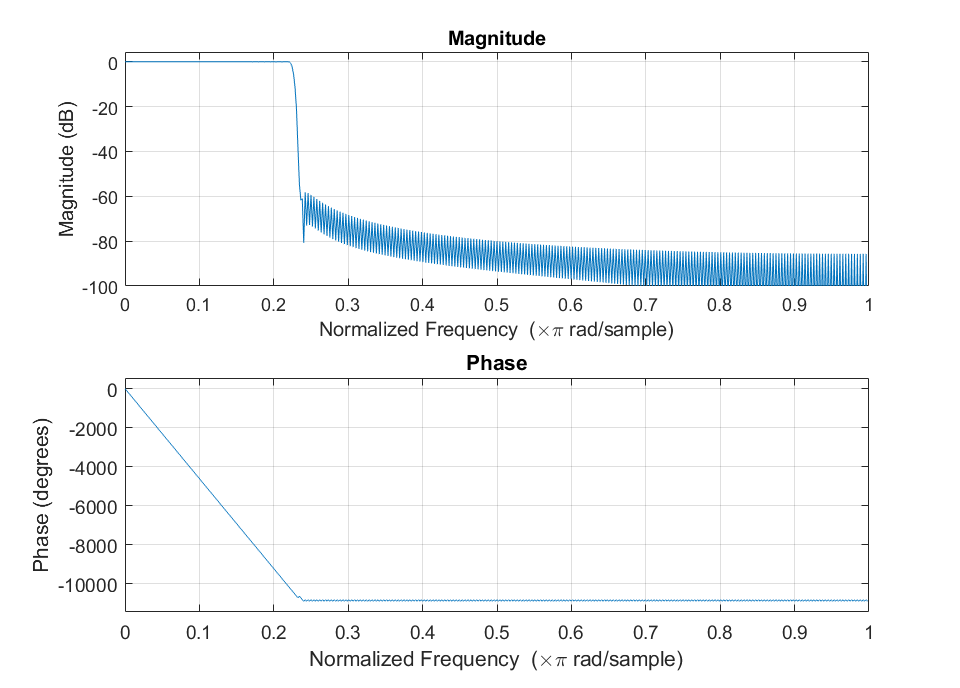
\includegraphics[width=13cm]{images/q1_b.png}
  \caption{Plot of the Frequency Response of the Low-Pass FIR filter.}
\end{figure}
\noindent Given the audio file \textit{love\_mono22.wav} the script below reads the audio file, passes it through
the FIR filter, and calculates the output signal:
\begin{lstlisting}[style=Matlab-editor, basicstyle=\small\ttfamily]
  figure(2);
  % Read audio file
  [x, Fs] = audioread('love_mono22.wav');

  % Filter the audio signal
  x_filtered = filter(filter_coeff, 1, x);

  % Plot the inputs power spectral density
  subplot(2, 1, 1);
  pwelch(x, [], [], [], Fs);
  title('Power Spectrum of Input Signal');

  % Plot the outputs power spectral density
  subplot(2, 1, 2);
  pwelch(x_filtered, [], [], [], Fs);
  title('Power Spectrum of Filtered Signal');

  % Create output file
  audiowrite('filtered_love_mono22.wav', x_filtered, Fs);
\end{lstlisting}
The script above produced the following power spectral density plots:
\begin{figure}[H]
  \centering
  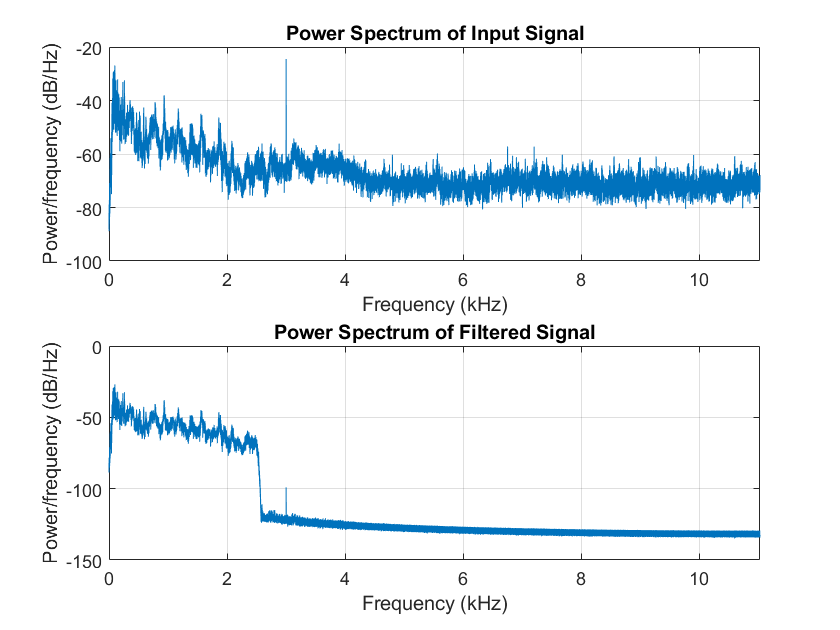
\includegraphics[width=13cm]{images/q1_e.png}
  \caption{Power Spectrums of Input (top) and Output (bottom) Signals.}
\end{figure}
Listening to the original and filtered signals it is clear that the filtered signal is now bass heavy in comparison
to the input signal. This is because the low-pass filter attenuates high frequency signals while passing low frequency
signals attributed to bass. Its also clear that the constant tone that can be heard throughout the song was filtered
significantly as it's much less noticeable in the output signal. This is supported by analyzing the power spectrums of
both signals. While there is a clear peak at approximately 3 kHz in the input signal, this peak is drastically reduced
in the output signal.

% Q2: High-Pass Filtering Audio Signals
\section{High-Pass Filtering Audio Signals}
The script below creates a 513-tap high-pass FIR filter with a cut-off frequency of 5000 Hz and a sampling frequency 5000
22050 Hz. The truncation window was selected to ensure that the stop-band ripples of the frequency response did not 
exceed -50dB. It then once again reads the \textit{love\_mono22.wav} audio file, passing its signal into the high-pass filter, 
and plotting the power density spectrums. Finally the new signal is outputted to a new \textit{filtered\_love\_mono22.wav} file:
\begin{lstlisting}[style=Matlab-editor, basicstyle=\small\ttfamily]
  figure(1);
  fc = 5000;              % Cutoff frequency in Hz
  Fs = 22050;             % Sampling frequency in Hz
  wc = fc / (Fs / 2);     % Normalized cutoff frequency

  % Windowing parameters
  window = hamming(513);   % Hamming window of length 513

  % Design the FIR filter using the fir1 function
  filter_coeff = fir1(513 - 1, wc, 'high', window); % 513 taps, 513 - 1 in the order

  % Plot the frequency response of the filter
  freqz(filter_coeff, 1); % 1024 points for a smooth plot, Fs as sampling frequency

  figure(2);
  % Read audio file
  [x, Fs] = audioread('love_mono22.wav');

  % Filter the audio signal
  x_filtered = filter(filter_coeff, 1, x);

  % Plot the inputs power spectral density
  subplot(2, 1, 1);
  pwelch(x, [], [], [], Fs);
  title('Power Spectrum of Input Signal');

  % Plot the outputs power spectral density
  subplot(2, 1, 2);
  pwelch(x_filtered, [], [], [], Fs);
  title('Power Spectrum of Filtered Signal');

  % Create output file
  audiowrite('filtered_love_mono22.wav', x_filtered, Fs);
\end{lstlisting}
The code above generates the following frequency response plots:
\begin{figure}[H]
  \centering
  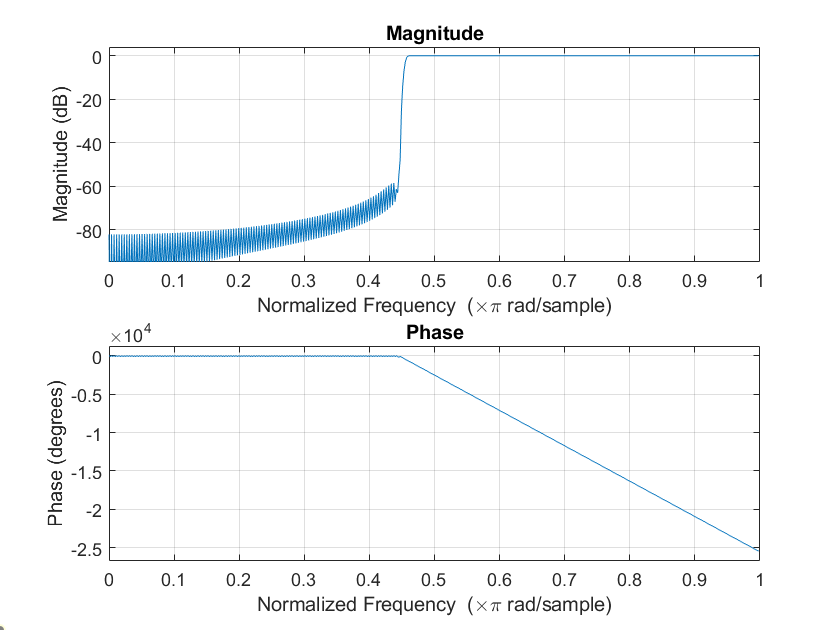
\includegraphics[width=13cm]{images/q2_b.png}
  \caption{Plot of the Frequency Response of the High-Pass FIR filter.}
\end{figure}
\noindent And the following power density spectrums:
\begin{figure}[H]
  \centering
  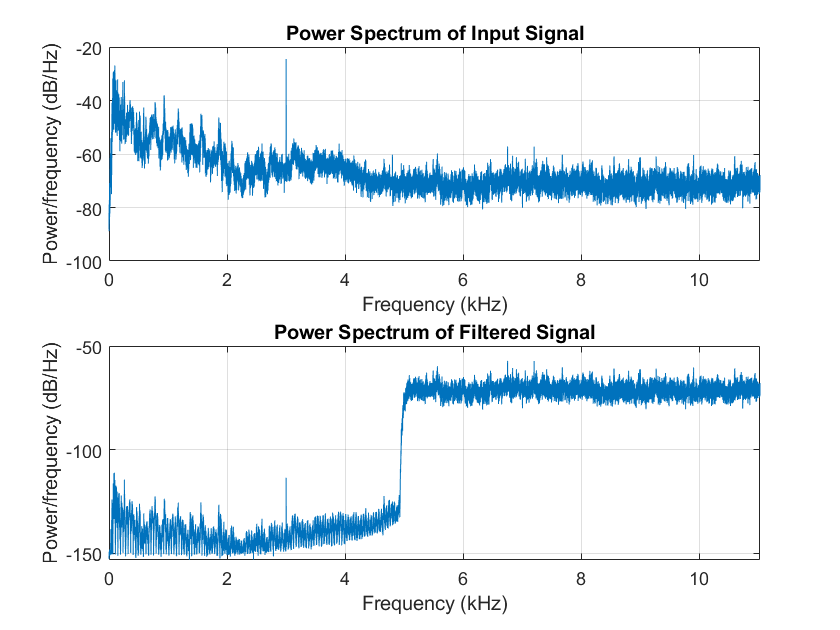
\includegraphics[width=13cm]{images/q2_e.png}
  \caption{Power Spectrums of the Input (top) and Output (bottom) Signals.}
\end{figure}
\noindent The filtered audio signal is almost unrecognizable to the input signal. There vocals and bass have been nearly completely
attenuated. The only recognizble elements from the original signal are the high frequency elements of the instrumentals.
Similar to the low-pass filter, the constant tone that can be heard throughout the song was filtered
significantly as it's much less noticeable in the output signal. This is supported by analyzing the power spectrums of
both signals. While there is a clear peak at approximately 3 kHz in the input signal, this peak is drastically reduced
in the output signal.
  
% Q2: High-Pass Filtering Audio Signals
\section{Audio Signal Filter Design}
In order to filter out the constant tone without negatively affecting other aspects of the audio signal, it was passed through
a band-stop filter per the script below:
\begin{lstlisting}[style=Matlab-editor, basicstyle=\small\ttfamily]
  figure(1);
  fc_lower  = 2900;                    % Lower cutoff frequency in Hz
  fc_upper = 3100;                     % Upper cutoff frequency in Hz
  Fs = 22050;                          % Sampling frequency in Hz
  wc_lower = fc_lower  / (Fs / 2);     % Normalized lower cutoff frequency
  wc_upper = fc_upper / (Fs / 2);      % Normalzied upper cutoff frequencyi

  % Windowing parameters
  window = hamming(513);   % Hamming window of length 513

  % Design the FIR filter using the fir1 function
  filter_coeff = fir1(513 - 1, [wc_lower wc_upper], 'stop', window); % 513 taps, 513 - 1 in the order

  % Plot the frequency response of the filter
  freqz(filter_coeff, 1); % 1024 points for a smooth plot, Fs as sampling frequency

  figure(2);
  % Read audio file
  [x, Fs] = audioread('love_mono22.wav');

  % Filter the audio signal
  x_filtered = filter(filter_coeff, 1, x);

  % Plot the inputs power spectral density
  subplot(2, 1, 1);
  pwelch(x, [], [], [], Fs);
  title('Power Spectrum of Input Signal');

  % Plot the outputs power spectral density
  subplot(2, 1, 2);
  pwelch(x_filtered, [], [], [], Fs);
  title('Power Spectrum of Filtered Signal');

  % Create output file
  audiowrite('filtered_love_mono22.wav', x_filtered, Fs);
\end{lstlisting}
The code above generates the following frequency response plots:
\begin{figure}[H]
  \centering
  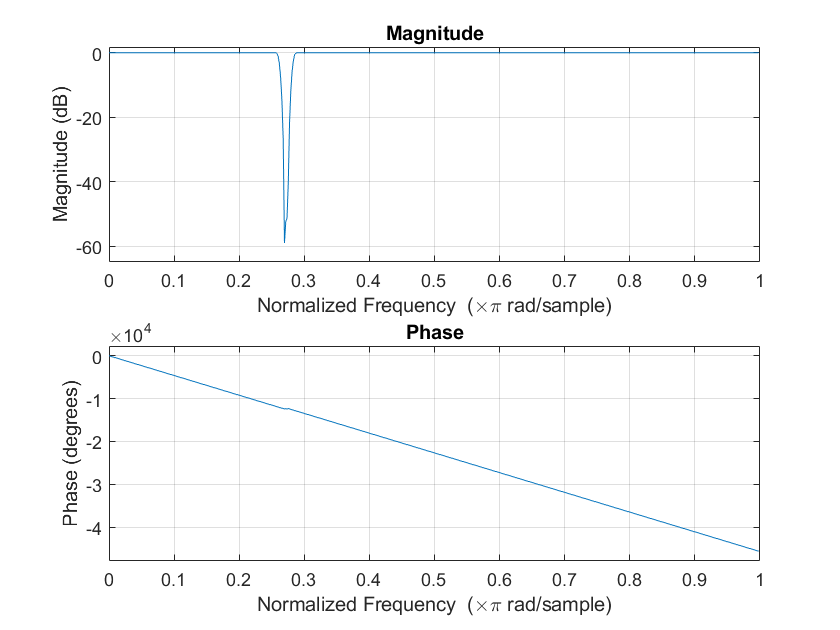
\includegraphics[width=13cm]{images/q3_c.png}
  \caption{Plot of the Frequency Response of the Band-Stop FIR filter.}
\end{figure}
And the following power density spectrums:
\begin{figure}[H]
  \centering
  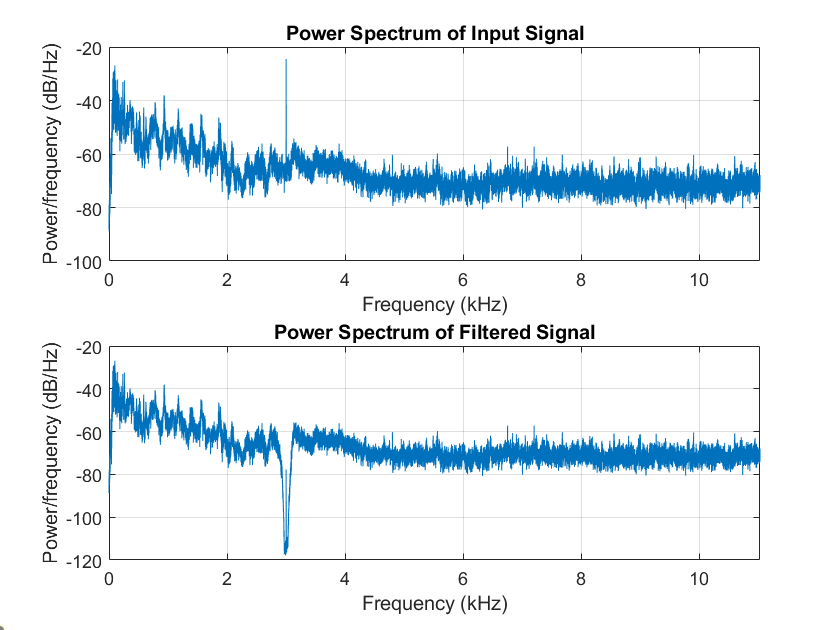
\includegraphics[width=13cm]{images/q3_e.png}
  \caption{Plot of the Power Spectrums of the Input (top) and Output (bottom) Signals.}
\end{figure}
\noindent Listening to the output signal, the tone is substantially attenuated while there are no audible effects on the rest
of the recording. This is also visible on the power density spectrum of the output where it is clear that the peak at 3 khz is 
attenuated significantly.

% Q4 : Filtering Image Files 
\section{Filtering Noisy Images}
Given the image file \textit{ayantika.tif}:
\begin{figure}[H]
  \centering
  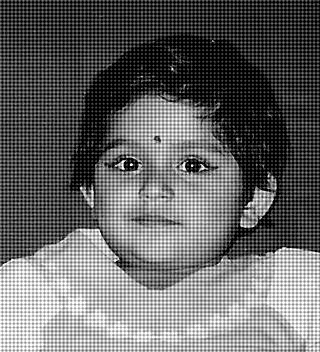
\includegraphics[width=6cm]{images/q4_ayantika.png}
  \caption{Original \textit{ayantika.tif} Image.}
\end{figure}
The code below filters the image and plots the power spectrums of the input and output images:
\begin{lstlisting}[style=Matlab-editor, basicstyle=\small\ttfamily]
  % MATLAB code for spectral analysis and lowpass filtering of an image
  % see section 17.6, Fig. 17.20, Fig. 17.21
  %
  % reading the image 'ayantika.tif'
  I = imread('ayantika.tif');
  Iu=I;     % copy of original image
  imshow(I)                   % display the image
  fprintf('\nThe image Ayantika has been displayed')
  fprintf('\nPress any key to continue')
  pause
  I = double(I);
  I = I - mean(mean(I));
  % 2D Bartlett window
  x = bartlett(32);
  for i = 1:32
      zx(i,:) = x';
    zy(:,i) = x ;
  end
  bartlett2D = zx .* zy;
  %
  n = 0;
  % calculate power spectrum
  P = zeros(256,256);
  for (i = 1:16:320)
      for (j = 1:16:288)
          Isub = I(i:i+31,j:j+31).*bartlett2D;
          P = P + fftshift(fft2(Isub,256,256));
          n = n + 1;
      end
  end
  Pabs = (abs(P)/n).^2;
  mesh([-128:127]*2/256,[-128:127]*2/256,Pabs/max(max(Pabs)));
  xlabel('Horizontal Frequency'); ylabel('Vertical Frequency');
  zlabel('Image Power Spectrum (in dB)');
  print -dtiff plot1.tiff
  fprintf('\nThe Image Power Spectrum has been displayed and saved')
  fprintf('\nPress any key to continue')
  pause

  filter_coeff = [1  2 3 2 1; 2  3  4  3 2; 3  4  5  4 3; 2  3  4  3  2; 1  2  3  2 1]/65 ;
  % Frequency Response plot
  spec = fft2(filter_coeff,128,128) ;     % Frequency spectrum of 2-D Filter
  R = abs(spec(1:65,1:65)) ;
  mesh(R), grid
  xlabel('Horizontal Frequency')
  ylabel('Vertical Frequency');
  zlabel('Frequency Response');
  print -dtiff plot.tiff
  fprintf('\nThe Frequency Response of the 2-D Filter has been displayed and saved')
  fprintf('\nPress any key to continue')
  pause
  %
  % Digital filtering the image
  filtered_image = filter2(filter_coeff, double(I)) ;
  imshow(uint8(filtered_image))
  %imshow(Iu)
  imwrite(uint8(filtered_image),'ayantika_filt.tif','tif') ;
  fprintf('\nThe Filtered Image has been displayed and saved')
\end{lstlisting}
The script above returns the following plots and images:
\begin{figure}[H]
  \centering
  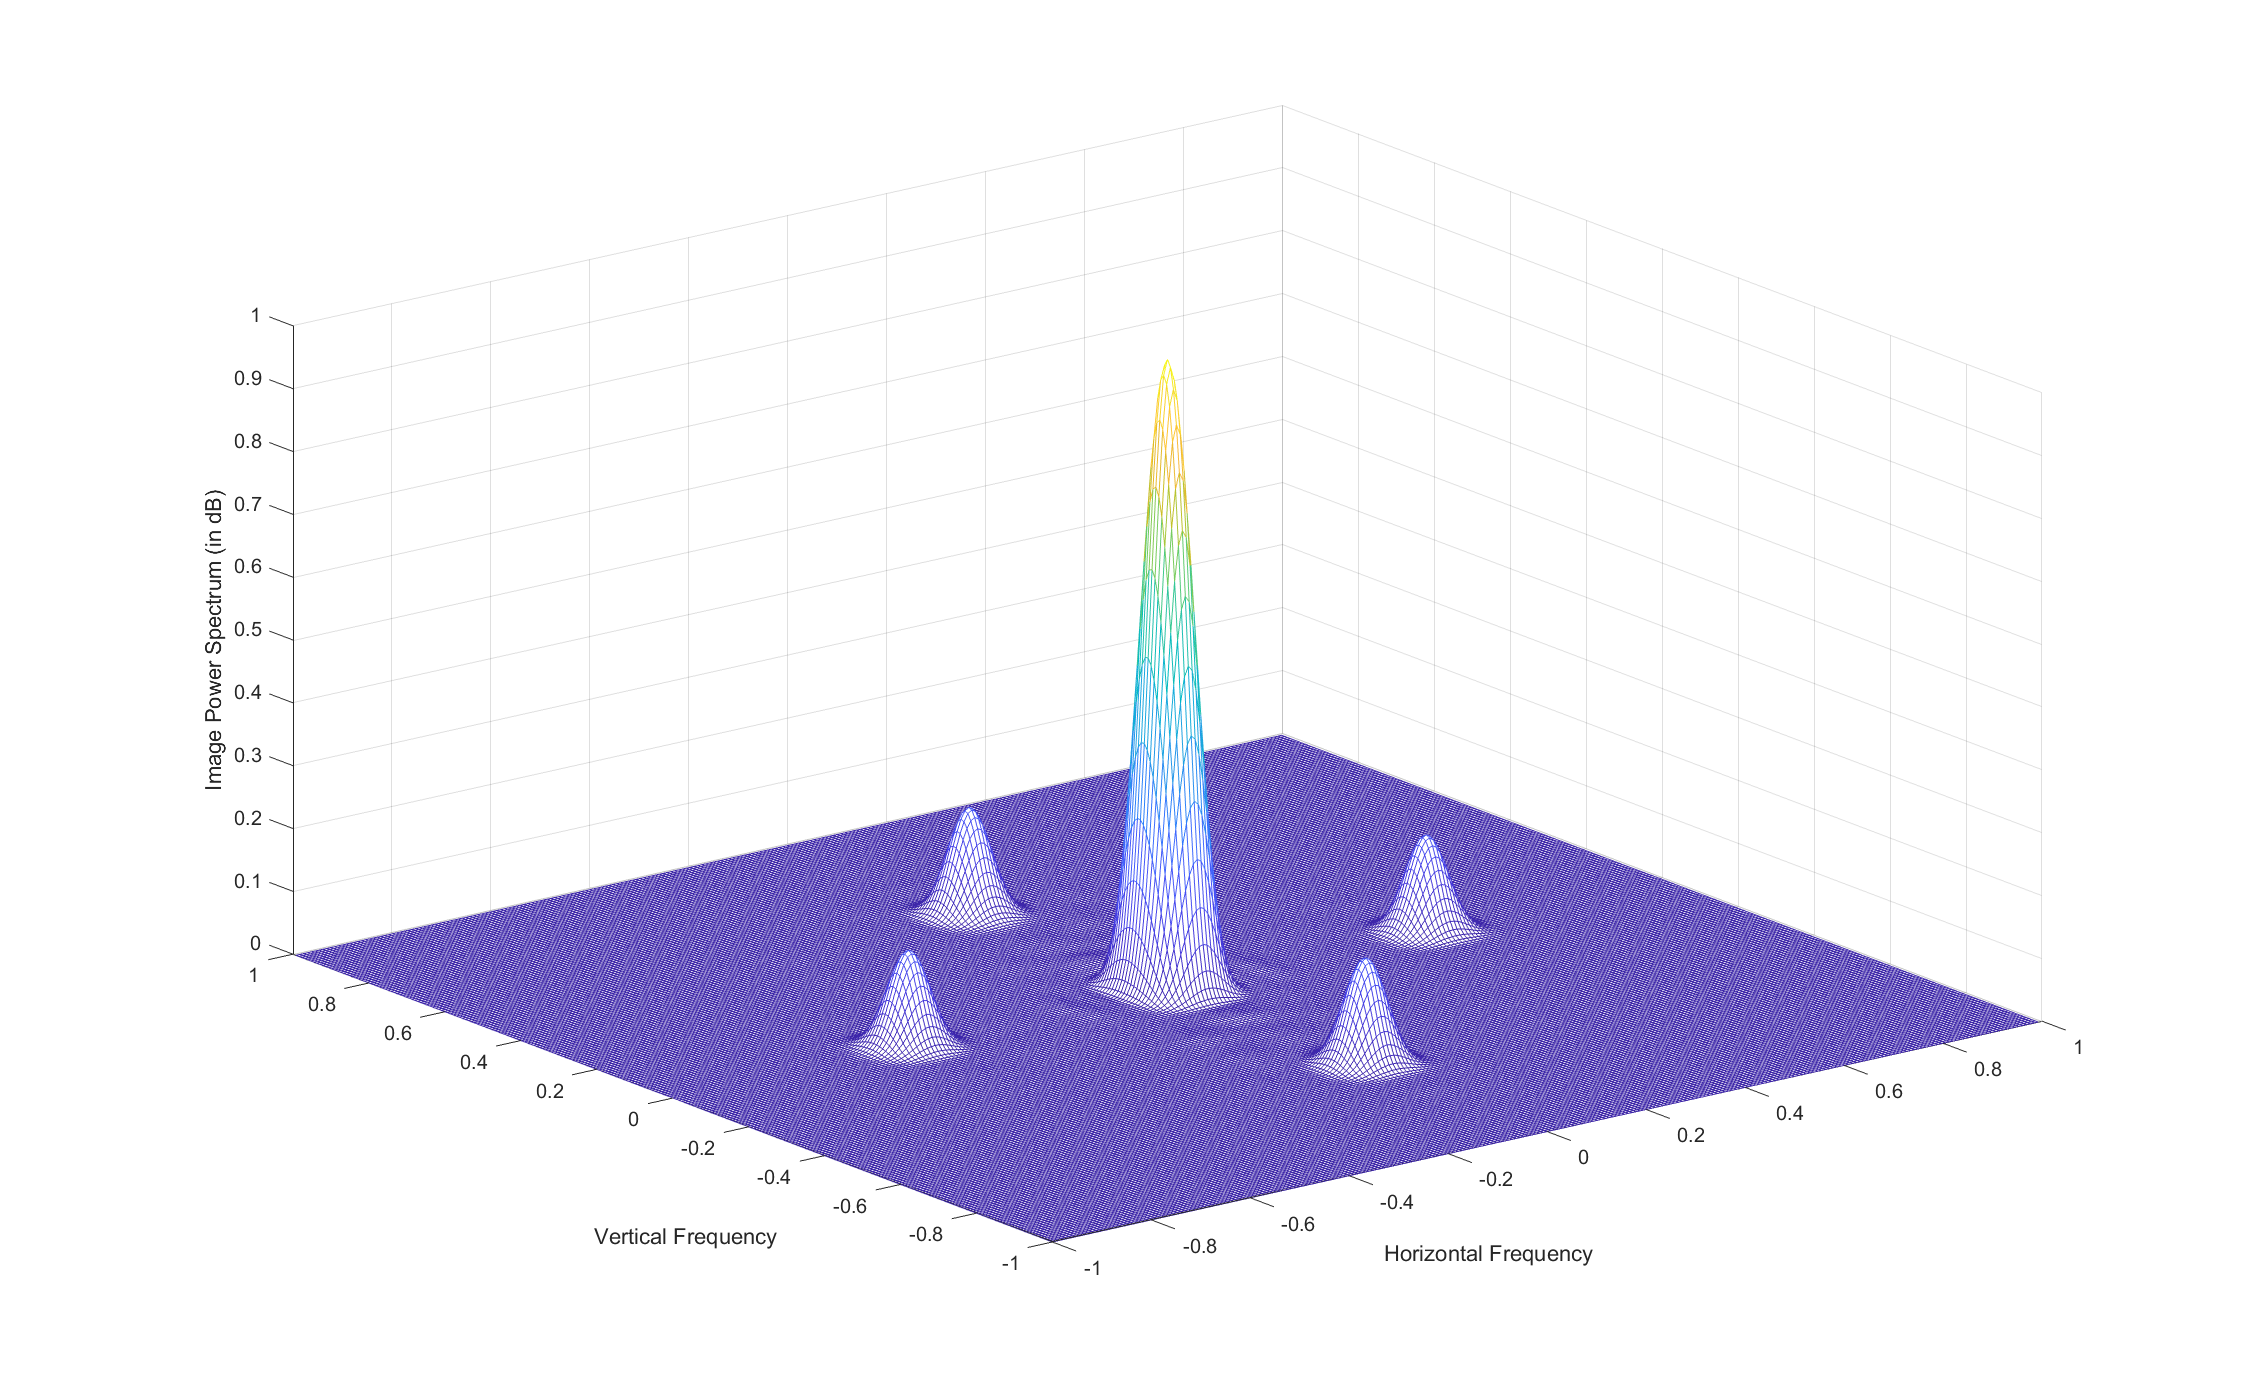
\includegraphics[width=16cm]{images/q4_b1.png}
  \caption{Plot of the Power Spectrum of the Input Image.}
\end{figure}
\begin{figure}[H]
  \centering
  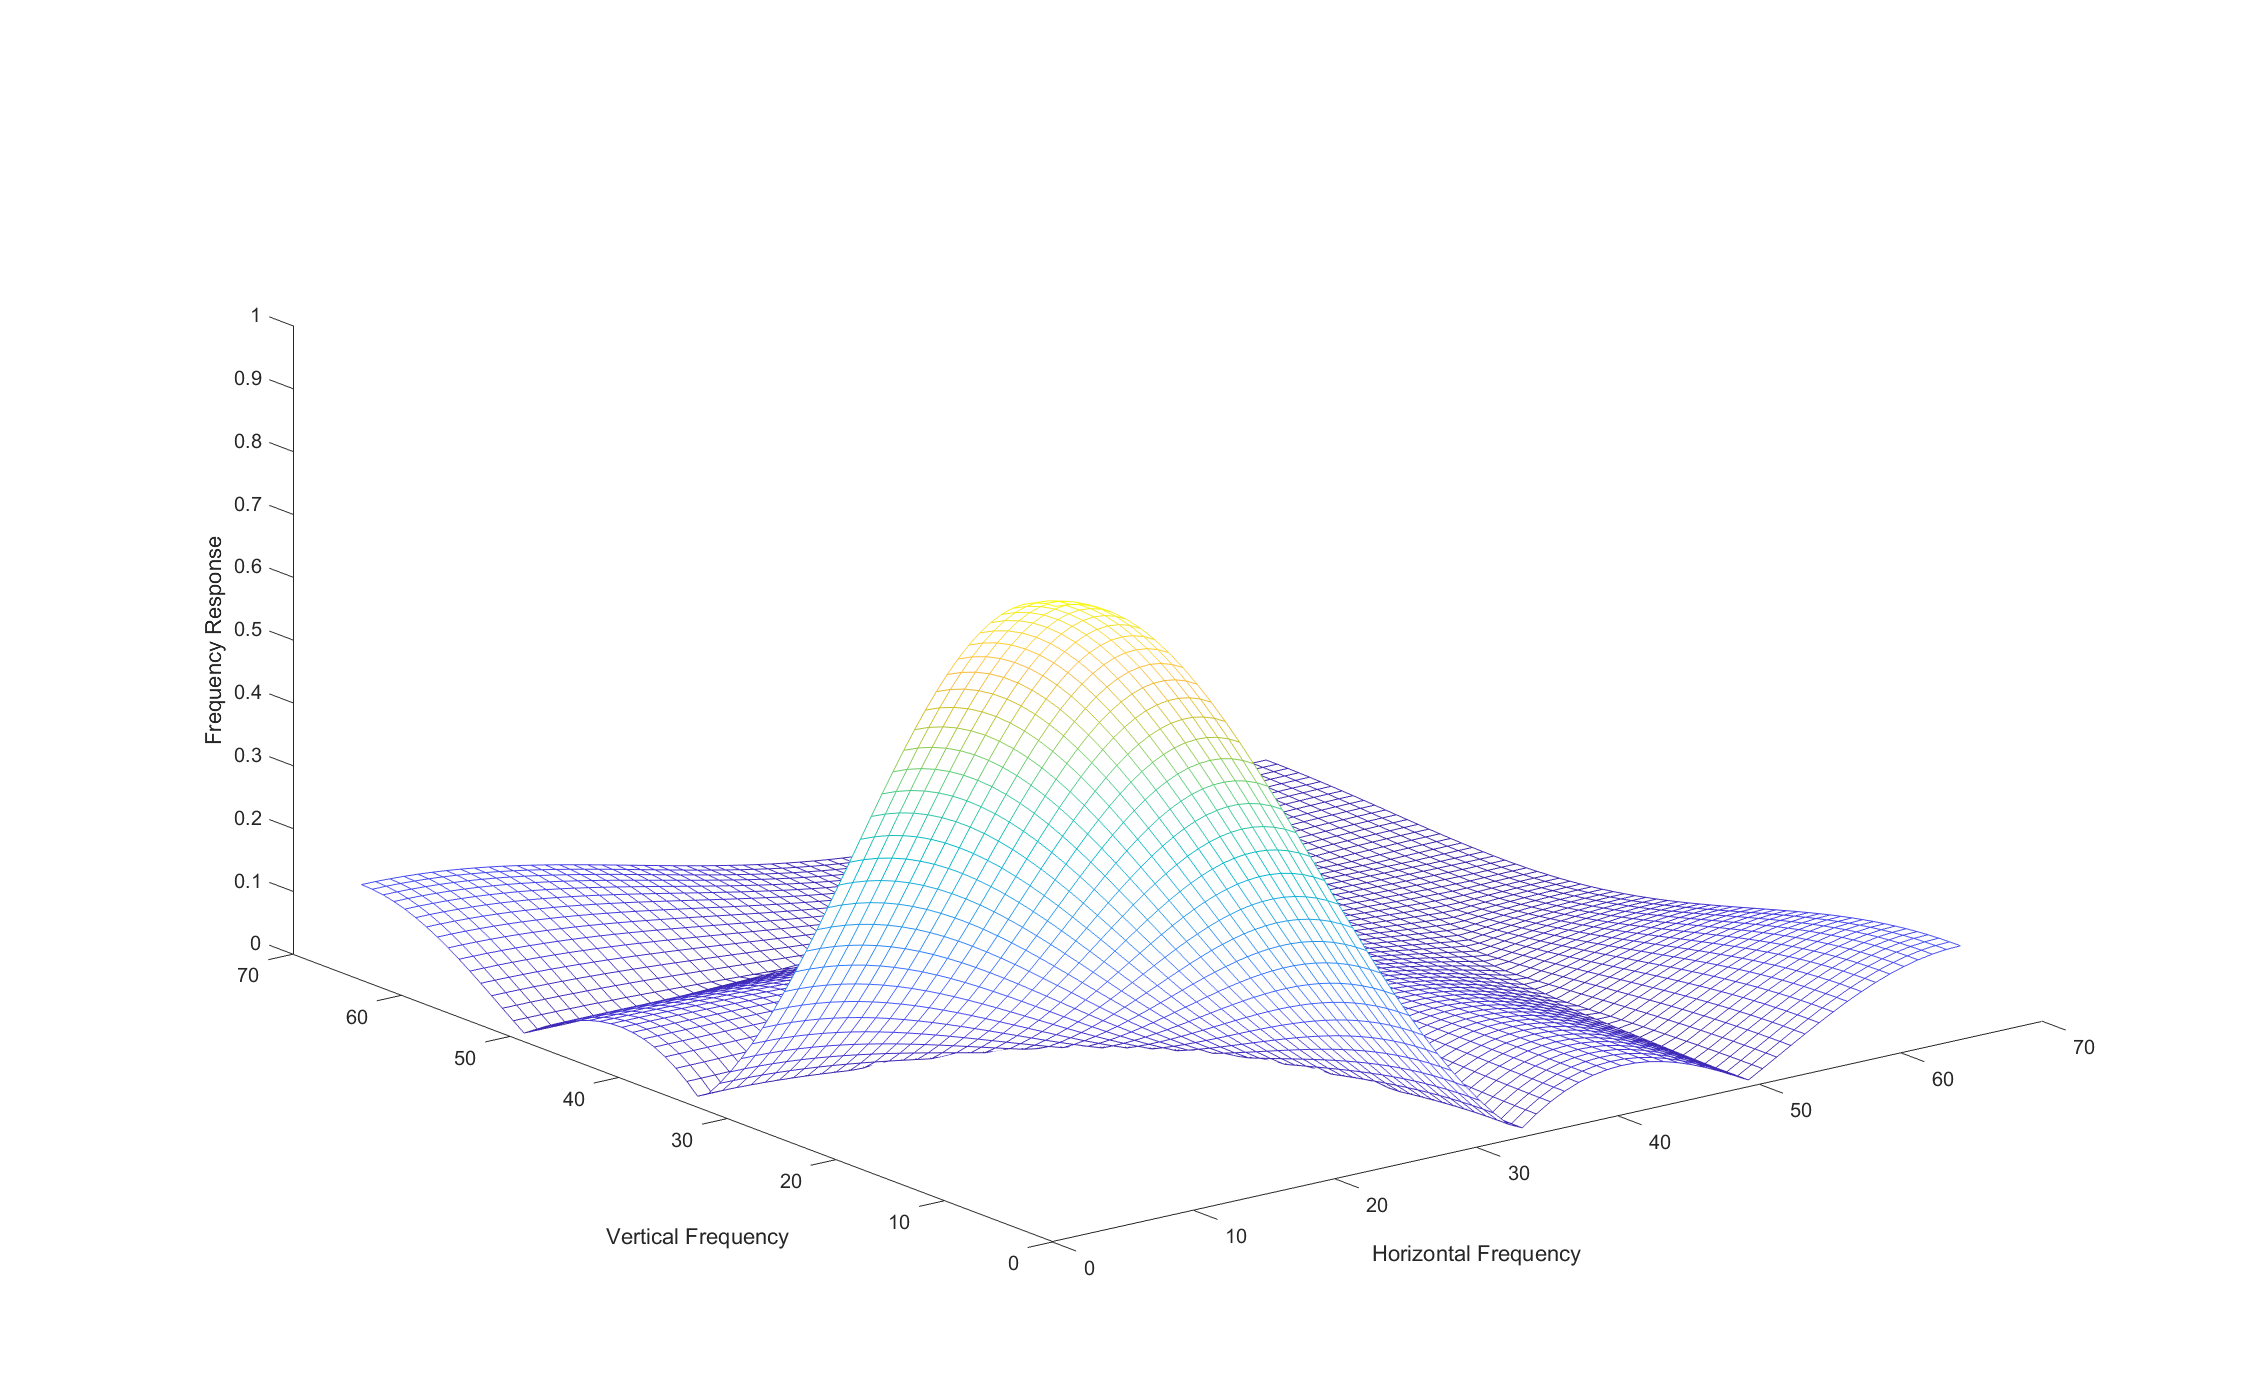
\includegraphics[width=16cm]{images/q4_b2.png}
  \caption{Plot of the Power Spectrum of the Output Image.}
\end{figure}
\begin{figure}[H]
  \centering
  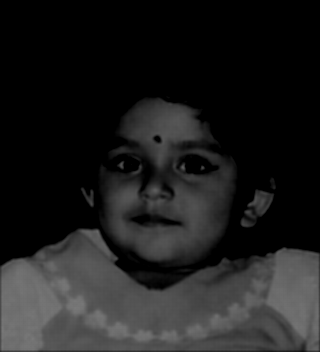
\includegraphics[width=6cm]{images/q4_ayantika_filt.png}
  \caption{\textit{ayantika.tif} After Filtering.}
\end{figure}
\noindent The input image had a very prominent grid like artifact which seperated the shaded pixels apart. The power spectrum showed 
the peaks/nodes that created the artifact. Applying a low-pass filter resulted in an image where lower frequency darker
shades are more prominent, and all higher frequency lighter shades are attenuated.
\end{document}